\chapter{插讲续篇：从反常层到D模}\label{L14}\lecturedate{2020/04/01}\sourcepage{115}
对复代数流形，复向量空间层的有界可构造复形的导出范畴，等价于上同调为正则完整D模的有界复形的导出范畴。特别地，在这一等价下，正则完整D模恰好对应于复系数反常层。这就是\textbf{Riemann--Hilbert对应}\znote{Riemann--Hilbert 对应是解析 D 模与拓扑层之间的桥。最经典的形式说：复流形上的平坦向量丛（等价于局部系统）与基本群的有限维复表示一一对应；一般形式则把正则完整 D 模的导出范畴与复系数可构造层（反常层）的导出范畴等价起来，由 Mebkhout 与 Kashiwara 独立证明。[来源：nLab 「Riemann-Hilbert correspondence」，\url{https://ncatlab.org/nlab/show/Riemann-Hilbert+correspondence}（Last revised 2024-08-09；2026-11-14 访问）。]}。因此，在Langlands纲领的复几何情形中，可以用D模替代反常层。

本讲简要介绍D模\znote{D模（D-module）是微分算子层 $\mathcal D_X$ 上的模层。局部取坐标 $x_1,\dots,x_{d_X}$ 时，$\mathcal D_X$ 由 $\OO_X$ 与 $\partial_1,\dots,\partial_{d_X}$ 生成，并满足 Weyl 代数关系 $[\partial_i,x_j]=\delta_{ij}$。因此 D模是带可积联络的向量丛的推广：它允许有奇点，也允许非局部自由的系数。D模之间的态射是 $\mathcal D_X$-线性的层同态，整体截面自然构成 $\mathcal D_X(X)$-模。[来源：J. Bernstein, \textit{Algebraic Theory of D-modules}（本讲参考文献 [B]）；并见 nLab 「D-module」，\url{https://ncatlab.org/nlab/show/D-module}（Last revised 2024-07-27；2026-11-14 访问）。]}。除非另有说明，本讲始终采用解析情形：$X$为复流形，$\OO_X$为$X$上的全纯函数层。
\section{D模}\label{L14S1}\idx{D模}\idx{微分算子}\idx{可积联络}
如下定义$X$上的微分算子层$\mathcal D_X$。对任意开集$U\subseteq X$，$U$上的\textbf{微分算子}是$P\in\End_{\C}(\OO_X(U))$，其阶数递归定义为：
\begin{itemize}
\item 若$P$为乘以某个函数$g\in\OO_X(U)$的算子，即对所有$f\in\OO_X(U)$有$P(f)=gf$，则$P$的阶数为零。
\item 对正整数$m$，若对所有$g\in\OO_X(U)$，算子$f\mapsto P(gf)-gP(f)$的阶数均不超过$m-1$，则$P$的阶数不超过$m$。
\end{itemize}
\sourcepage{116}
\originalnumber{1}
\begin{example}\label{L14S1O1}
若$P$的阶数为一，则按定义，$P(gf)-gP(f)$的阶数为零，因而是乘以某个函数$g'$的算子。于是
\[\begin{aligned}
P(gf)-gP(f)&=g'f&&\text{对所有 }f,g\in\OO_X(U),\\
P(g)-gP(1)&=g',\\
P(gf)-fP(g)&=gP(f)-fgP(1),
\end{aligned}\]
其中$1$为处处取值为$1$的常值函数。

因此，算子$\widetilde P:=P-P(1)\cdot$，即$\widetilde P(f)=P(f)-P(1)f$，满足Leibniz法则
\[\widetilde P(fg)=g\widetilde P(f)+f\widetilde P(g).\]
此外，$\widetilde P(\C)=0$，这里$\C$表示所有常值函数。
\end{example}
由$X$上全部微分算子组成的层$\mathcal D_X$，具有按算子阶数给出的滤过：
\[\OO_X\cong F_0\mathcal D_X\subseteq\cdots\subseteq F_m\mathcal D_X\subseteq F_{m+1}\mathcal D_X\subseteq\cdots\subseteq\mathcal D_X=\bigcup_{m\ge0}F_m\mathcal D_X\subseteq\mathcal End_{\C}(\OO_X).\]
其中$F_m\mathcal D_X$为阶数不超过$m$的算子层。
\originalnumber{2}
\begin{note}[L14S1O2]
$\mathcal D_X$是$\OO_X$-模层，通常并不凝聚\znote{$\mathcal D_X$ 局部由无穷多个偏导 $\partial^\alpha$ 生成，作为 $\OO_X$-模不是有限生成的，因此一般不是凝聚 $\OO_X$-模（它是拟凝聚的）。这里说的「不凝聚」针对 $\OO_X$-模结构，与后文「$\mathcal D_X$ 是凝聚 $\mathcal D_X$-模」并不矛盾：两者用的是不同的模结构。[来源：Peters--Steenbrink, \textit{Mixed Hodge Structures}, Ch. 13 §13.3--§13.6（本讲参考文献）。]}；在代数情形中，它是拟凝聚的$\OO_X$-模层。
\end{note}

\originalnumber{3}
\begin{definition}\label{L14S1O3}
左$\mathcal D_X$-模层$\mathcal F$称为\textbf{$\mathcal D_X$模}；在不致混淆时，简称\textbf{D模}。
\end{definition}
\originalnumber{4}
\begin{lemma}\label{L14S1O4}
设$\mathcal F$为$\OO_X$-模层。下列两种结构一一对应：
\begin{enumerate}[label=(\alph*)]
\item $\mathcal F$上的左$\mathcal D_X$-模结构；
\item 保持Lie括号的$\OO_X$-线性映射
\[\rho:T_X\longrightarrow\mathcal End_{\C}(\mathcal F),\]
且满足Leibniz法则$\rho(\theta)(hu)=\theta(h)u+h\rho(\theta)u$，其中$h,\theta,u$分别为$\OO_X,T_X,\mathcal F$的局部截面，$T_X$为$X$的切丛。
\end{enumerate}
特别地，若$\mathcal F$作为$\OO_X$-模层局部自由，则这些结构对应于$\mathcal F$上的可积联络\znote{「可积」指联络的曲率为零，所以可积联络也叫平坦联络（flat connection）；局部坐标下曲率为零等价于 $\nabla_i\nabla_j=\nabla_j\nabla_i$。平坦性保证平行移动只依赖路径的同伦类，这正是平坦联络与局部系统（局部常值层）彼此等同的原因；对不平坦的联络，平行移动会依赖路径本身。[来源：nLab 「flat connection」，\url{https://ncatlab.org/nlab/show/flat+connection}（Last revised 2023-06-04；2026-11-14 访问）。]}，即与Lie括号相容的联络。
\end{lemma}
\sourcepage{117}
\originalnumber{5}
\begin{note}[L14S1O5]
非零且作为$\OO_X$-模为拟凝聚的D模，其局部湮灭理想为零：在非零茎处，不存在一个非零的全纯函数芽将整个模湮灭。事实上，若$f$湮灭整个模，D模结构以及Leibniz法则说明$f$的各阶偏导也湮灭整个模。在局部坐标中选取适当阶数的偏导，可使所得函数在该点非零；缩小邻域并乘以其倒数，便得到常数$1$也湮灭该模，矛盾。
\end{note}
$\mathcal D_X$是非交换环层，因此左$\mathcal D_X$模与右$\mathcal D_X$模的结构并不相同。设$\Omega_X^1$为$X$上的微分形式层，$\Omega_X^n:=\bigwedge^n\Omega_X^1$；特别地，令$\omega_X:=\Omega_X^{d_X}$，其中$d_X=\dim_{\C}X$。$T_X$通过Lie导数作用于$\Omega_X^n$。这些作用一般不是联络，因为对$\OO_X,T_X,\Omega_X^n$的局部截面$f,\xi,w_n$，通常有
\[\mathcal L_{f\xi}(w_n)\ne f\mathcal L_\xi(w_n).\]
所以Lie导数一般不能赋予$\Omega_X^n$左D模结构。不过，在$\omega_X$上有$\mathcal L_{f\xi}(w)=\mathcal L_\xi(fw)$\znoteplain{原书此处表述含混（以下为提示，不是改写）：作为算子，Lie 导数对系数函数是线性的，即 $\mathcal L_{f\xi}=f\mathcal L_\xi$；但它作用在函数与微分形式以后，$\mathcal L_\xi(fw)=f\mathcal L_\xi(w)+(\xi f)w$，多出的 $(\xi f)w$ 正是右模与左模修正项的来源。原书这句应理解为：先约定 $w$ 为右模元，或已把该附加项吸收进作用定义，之后的简写。（上下文推断，无外部依据）}。这使$\omega_X$具有右D模结构，相应的切向量作用为
\[w\xi:=-\mathcal L_\xi(w)=-d\langle\xi,w\rangle.\]
% [Tutor Note: 原书 p117 此式作 $(\xi,w)\mapsto d\langle\xi,w\rangle$（无负号），译文按右 D 模结构的正确符号写作 $-\mathcal L_\xi(w)=-d\langle\xi,w\rangle$。]

现在可以在左D模和右D模之间作典范变换。这两种操作称为\textbf{左右变换}和\textbf{右左变换}，定义如下：
\begin{figure}[H]\centering
\begin{equation}\tag{1.1}\label{L14eq11}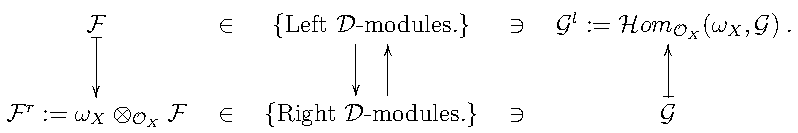
\includegraphics[width=0.6434\paperwidth]{images/L14-p117-leftright.pdf}\end{equation}
\end{figure}
$T_X$在$\omega_X\otimes_{\OO_X}\mathcal F$和$\mathcal Hom_{\OO_X}(\omega_X,\mathcal G)$上的作用分别为
\[(w\otimes u)\xi:=w\xi\otimes u-w\otimes\xi u,\qquad (\xi\varphi)(w):=\varphi(w\xi)-\varphi(w)\xi.\]
若$\mathcal G$为右D模，也称它为$\mathcal D^r$模；不加说明的D模始终指左D模。将$\mathcal D$自身视为右D模时，记为$\mathcal D^r$。

以$\mu(\mathcal D_X)$表示$\mathcal D_X$模的范畴，则有：
\originalnumber{6}
\begin{proposition}\label{L14S1O6}
$\mu(\mathcal D_X)$具有足够多的内射对象\znote{内射对象 $I$ 的性质是：对任意单射 $A\hookrightarrow B$ 与任意映射 $A\to I$，都存在 $B\to I$ 使之延拓。「足够多内射对象」意味着每个模都能嵌入某个内射模，这是 $\mathrm{RHom}$ 与导出范畴的整套同调代数能在 $\mu(\mathcal D_X)$ 中运作的前提；同调维数不超过 $2\dim_{\C}X$ 则说明可以用长度有界的复形计算导出函子。[来源：nLab 「injective object」，\url{https://ncatlab.org/nlab/show/injective+object}（Last revised 2025-12-24；2026-11-14 访问）。]}和局部投射对象，其同调维数有限，不超过$2\dim_{\C}X$。
\end{proposition}
\sourcepage{118}
可以类似地定义D模的导出范畴$D(\mathcal D_X)$。以$D^b(\mathcal D_X)$表示有界D模复形的导出范畴。
若D模$\mathcal F$作为$\OO_X$-模层局部自由，则有以下$\C_X$-线性复形：
\begin{equation}\tag{1.2}\label{L14eq12}
\operatorname{DR}_X(\mathcal F)=\bigl(\mathcal F\to\Omega_X^1\otimes\mathcal F\to\cdots\to\Omega_X^{d_X}\otimes\mathcal F\bigr)[d_X].
\end{equation}
% [Tutor Note: 原书 p118 作 $\Omega_X^{d_X-1}\otimes\mathcal F$，译文按 de Rham 复形的正确末项 $\Omega_X^{d_X}$ 处理。]
其中微分由\eref{引理}{L14S1O4}中D模结构对应的可积联络给出。\eqref{L14eq12}中的复形称为$\mathcal F$的\textbf{de Rham复形}，记为$\operatorname{DR}_X(\mathcal F)$。利用$\omega_X$的局部自由右$\mathcal D_X$-模消解，可得
\[\operatorname{DR}_X(\mathcal F)\cong\omega_X\overset{\mathrm L}{\otimes}_{\mathcal D_X}\mathcal F.\]
因此，对有界D模复形，可以定义
\[\operatorname{DR}_X(\mathcal F^\bullet):=\omega_X\overset{\mathrm L}{\otimes}_{\mathcal D_X}\mathcal F^\bullet.\]
我们将看到，将D模送到它的de Rham复形，正是实现Riemann--Hilbert对应的方式。\idx{de Rham复形}

\textbf{对偶化左D模}为
\[\mathcal D_X^\vee:=\mathcal Hom_{\OO_X}(\omega_X,\mathcal D_X^r),\]
即通过右左变换从$\mathcal D_X^r$得到的左模。对左D模$\mathcal F$，利用这一双模定义其对偶模
\[\mathcal F^\vee:=\mathcal Hom_{\mathcal D_X}(\mathcal F,\mathcal D_X^\vee).\]
在导出范畴中再加入平移$[d_X]$，得到对偶函子
\[\mathbb D_X(\mathcal F^\bullet):=\mathrm R\mathcal Hom_{\mathcal D_X}(\mathcal F^\bullet,\mathcal D_X^\vee)[d_X].\]
有
\begin{equation}\tag{1.3}\label{L14eq13}
\operatorname{DR}_X(\mathbb D_X(\mathcal F^\bullet))\cong\mathrm R\mathcal Hom_{\mathcal D_X}(\mathcal F^\bullet,\OO_X)[d_X].
\end{equation}
还可以定义逆像和直像。对复流形之间的全纯映射$f:X\to Y$，逆像的底层$\OO_X$-模为
\[f^*\mathcal G:=\OO_X\otimes_{f^{-1}\OO_Y}f^{-1}\mathcal G.\]
\sourcepage{119}
直像定义为
\[f_+\mathcal F:=f_*\mathcal F\otimes_{\mathcal D_X}f^*\mathcal D_Y.\]
$f^*$和$f_+$诱导导出范畴之间的函子，仍使用相同记号；此时$f^*$中的张量积也取导出张量积\znoteplain{原书此处未给出转移双模的显式写法；易错点是 $f_+$ 与 $f^!$ 的方向：$f_+$ 沿 $f$ 推前，把左 $\mathcal D_X$-模送到左 $\mathcal D_Y$-模，而 $f^!$ 形式上由 $\mathbb D$ 与 $f_+$ 复合给出，方向与 $f_+$ 相反，两者并非同一方向上的函子；套用公式前须先确认所引文献的左右模手性约定，否则平移与对偶会整体错位。（上下文推断，无外部依据）}。令$f^!:=f^*\circ[d_X-d_Y]$，再用对偶算子定义另外两个函子：
% [Tutor Note: 原书 p119 作 $f^!:=f^*\circ[d_Y-d_X]$，而 p124 的交换图按相反约定（由 $\operatorname{DR}_X(\OO_X)\cong\C_X[d_X]$ 验算，需平移 $[d_Y-d_X]$），二者互相矛盾，属原书内部约定不统一；译文统一取 $f^*[d_X-d_Y]$（与译文 $\mathbb D_X=\mathrm R\mathcal Hom(-,\mathcal D_X^\vee)[d_X]$ 的对偶约定自洽），读者引用时须按所引文献的约定换算。]
\[f^+:=\mathbb D_X\circ f^!\circ\mathbb D_Y,\qquad f_!:=\mathbb D_Y\circ f_+\circ\mathbb D_X.\]
\originalnumber{7}
\begin{theorem}[Kashiwara]\label{L14S1O7}
设$i:Z\to X$为非奇异流形之间的闭嵌入。令$\mu_Z(\mathcal D_X)$为$\mu(\mathcal D_X)$中由支撑包含于$Z$的$\mathcal D_X$模组成的满子范畴。
% [Tutor Note: 原书 p119 此处将 $\mu_Z(\mathcal D_X)$ 误作 $\mu_Z(\mathcal D_Z)$（它与「$\mu(\mathcal D_X)$ 的满子范畴」矛盾），译文按正确写法处理。]则函子
\[i_+:\mu(\mathcal D_Z)\to\mu_Z(\mathcal D_X),\qquad i^+:\mu_Z(\mathcal D_X)\to\mu(\mathcal D_Z)\]
互为逆函子，给出范畴等价。
\end{theorem}
\originalnumber{8}
\begin{note}[L14S1O8]
\eref{定理}{L14S1O7}还可以帮助我们定义奇异闭子簇$Z$上的D模范畴；此时$\mathcal D_Z$本身可能相当难处理。只需将$\mu(\mathcal D_Z)$定义为$\mu(\mathcal D_X)$的满子范畴$\mu_Z(\mathcal D_X)$。
\end{note}
\section{凝聚D模与完整D模}\label{L14S2}\idx{凝聚D模}\idx{完整D模}\idx{良滤过}\idx{特征簇}
若$\mathcal D_X$模$\mathcal F$局部有限表示，即局部有限生成，并且关系模也局部有限生成，则称它\textbf{凝聚}。换言之，在某个开集$U\subseteq X$上有正合列
\begin{equation}\tag{2.1}\label{L14eq21}
\mathcal D_X(U)^q\xrightarrow{\alpha}\mathcal D_X(U)^p\longrightarrow\mathcal F(U)\longrightarrow0.
\end{equation}
\originalnumber{1}
\begin{note}[L14S2O1]
凝聚$R$模$M$是一个有限生成模，并且任意有限组生成元之间的关系模也有限生成。因此，当$A$也凝聚时，任意满射$M^p\twoheadrightarrow A$的核都是有限生成的。

在代数几何的Noether情形中，对拟凝聚模而言，凝聚性就是局部有限生成性。但在解析几何中，局部有限生成并不等价于局部有限表示，因为关系核未必局部有限生成。
\sourcepage{120}
例如，在Noether代数几何中，结构层$\OO_X$的凝聚性是直接的；解析几何中的$\OO_X$也凝聚，但这是Oka的一个深刻定理。

$\OO_X$作为$\OO_X$-模凝聚这一很不平凡的事实，推出$\mathcal D_X$作为左$\mathcal D_X$模凝聚。因此，$\mathcal D_X$模的凝聚性等价于局部有限表示性。
\end{note}
以$\mu_{\mathrm{coh}}(\mathcal D_X)$表示$\mu(\mathcal D_X)$中由凝聚$\mathcal D_X$模组成的满子范畴。若D模复形的所有上同调层均凝聚，就称该复形凝聚。以$D_{\mathrm{coh}}^b(\mathcal D_X)$表示$D^b(\mathcal D_X)$中由凝聚D模复形组成的满子范畴。
\originalnumber{2}
\begin{proposition}\label{L14S2O2}
$\mu_{\mathrm{coh}}(\mathcal D_X)$是阿贝尔范畴，自然函子
\[D^b(\mu_{\mathrm{coh}}(\mathcal D_X))\longrightarrow D_{\mathrm{coh}}^b(\mathcal D_X)\]
为范畴等价。
\end{proposition}
一般而言，凝聚D模的逆像或直像未必凝聚。不过有：
\originalnumber{3}
\begin{proposition}\label{L14S2O3}
若$f:X\to Y$为真态射，则$f_+(D_{\mathrm{coh}}^b(\mathcal D_X))\subseteq D_{\mathrm{coh}}^b(\mathcal D_Y)$。
\end{proposition}
回忆$\mathcal D_X$的滤过
\begin{equation}\tag{2.2}\label{L14eq22}
\OO_X\cong F_0\mathcal D_X\subseteq\cdots\subseteq F_m\mathcal D_X\subseteq F_{m+1}\mathcal D_X\subseteq\cdots\subseteq\mathcal D_X=\bigcup_{m\ge0}F_m\mathcal D_X,
\end{equation}
其中$F_m\mathcal D_X$为阶数不超过$m$的算子层。它满足$F_m\mathcal D_X\cdot F_n\mathcal D_X\subseteq F_{m+n}\mathcal D_X$。相关分次代数层记为
\[\operatorname{Gr}^{\mathrm{ord}}\mathcal D_X:=\bigoplus_mF_m\mathcal D_X/F_{m-1}\mathcal D_X.\]
它是交换的，并自然同构于余切丛$\Omega_X^1$上沿纤维为多项式、沿底空间为全纯函数的函数层。这里用相同记号表示局部自由层及其对应的向量丛。

对任意D模$\mathcal F$，其\textbf{滤过}是一个$\OO_X$-子模序列
\[\cdots\subseteq\mathcal F_0\subseteq\mathcal F_1\subseteq\cdots\subseteq\mathcal F_m\subseteq\cdots\subseteq\mathcal F,\]
\sourcepage{121}
满足$\mathcal F=\bigcup_{m\in\Z}\mathcal F_m$，且对所有$m\in\N,n\in\Z$有$F_m\mathcal D_X(\mathcal F_n)\subseteq\mathcal F_{m+n}$。若分次模$\operatorname{Gr}^F\mathcal F:=\bigoplus_m\mathcal F_m/\mathcal F_{m-1}$还是凝聚的$\operatorname{Gr}^{\mathrm{ord}}\mathcal D_X$模，则称滤过为\textbf{良滤过}。这等价于下列两条件同时成立：
\begin{enumerate}[label=\arabic*.]
\item 对所有$m\ll0$，$\mathcal F_m=0$；对所有$r\gg0$，$F_1\mathcal D_X(\mathcal F_r)=\mathcal F_{r+1}$；
\item 每个$\mathcal F_m$都是凝聚$\OO_X$模。
\end{enumerate}
每个凝聚$\mathcal D_X$模都局部具有良滤过。有如下结论。
\originalnumber{4}
\begin{proposition}\label{L14S2O4}
设$(\mathcal F,F)$为带有良滤过的凝聚$\mathcal D_X$模，以$\mathcal I(\mathcal F,F)$表示$\operatorname{Gr}^F\mathcal F$在$\operatorname{Gr}^{\mathrm{ord}}\mathcal D_X$中的湮灭理想。则$\sqrt{\mathcal I(\mathcal F,F)}$不依赖于$\mathcal F$上良滤过$F$的选取。
\end{proposition}
\eref{命题}{L14S2O4}中的理想层$\sqrt{\mathcal I(\mathcal F,F)}$定义余切丛$\Omega_X^1$的一个子簇，称为$\mathcal F$的\textbf{特征簇}\znote{特征簇是余切丛中的子簇，记录 $\mathcal F$ 的「奇异方向」：当特征簇落在某点的零纤维内时，$\mathcal F$ 在该点附近作为 $\OO_X$-模局部自由，即没有奇性。它由理想层的根定义，因而总是既约的；对完整 D 模，它还是余切丛的 Lagrange 子簇。[来源：nLab 「holonomic D-module」，\url{https://ncatlab.org/nlab/show/holonomic+D-module}（Last revised 2014-02-16；2026-11-14 访问）；并见 Peters--Steenbrink, \textit{Mixed Hodge Structures}, Ch. 13 §13.3--§13.6（本讲参考文献）。]}，亦称\textbf{奇异支撑}，记为$\operatorname{Char}(\mathcal F)$。注意，它恰好是$\operatorname{Gr}^F\mathcal F$作为凝聚$\operatorname{Gr}^{\mathrm{ord}}\mathcal D_X$模的支撑$\operatorname{Supp}(\operatorname{Gr}^F\mathcal F)\subseteq\Omega_X^1$。

一般很难描述逆像、直像的特征簇。$f_+,f^*$通常不保持D模的凝聚性。不过，对闭嵌入和光滑态射，有以下结果。
\begin{enumerate}[label=(\roman*)]
\item 若$i:Z\to X$为非奇异流形之间的闭嵌入，则对任意$\mathcal D_Z$模$\mathcal F$，$i_+\mathcal F$凝聚当且仅当$\mathcal F$凝聚。此外，
\[\operatorname{Char}(i_+\mathcal F)=\{(x,\xi)\mid x\in Z,\ (x,\operatorname{Pr}^{\Omega}(\xi))\in\operatorname{Char}(\mathcal F)\},\]
其中$\operatorname{Pr}^{\Omega}:\Omega_X^1|_Z\to\Omega_Z^1$为限制映射。
\item 若$\pi:Y\to X$为光滑态射，则微分给出映射$d\pi:\pi^*\Omega_X^1\to\Omega_Y^1$。对任意$\mathcal D_X$模$\mathcal G$，$\pi^*\mathcal G$凝聚当且仅当$\mathcal G$凝聚。此外，
\[\operatorname{Char}(\pi^*\mathcal G)=\{(y,\xi)\mid y\in Y,\ \xi=d\pi(\eta),\ (\pi(y),\eta)\in\operatorname{Char}(\mathcal G)\}.\]
\end{enumerate}
\originalnumber{5}
\begin{theorem}\label{L14S2O5}
若$\mathcal F\ne0$为凝聚$\mathcal D_X$模，则$\dim_{\C}\operatorname{Char}(\mathcal F)\ge\dim_{\C}X$。
\end{theorem}
\sourcepage{122}
\originalnumber{6}
\begin{definition}\label{L14S2O6}
若凝聚$\mathcal D_X$模$\mathcal F\ne0$满足$\dim_{\C}\operatorname{Char}(\mathcal F)=\dim_{\C}X$，则称它为\textbf{完整模}\znote{完整（holonomic）是 D 模理论中最基本的有穷性条件：它要求 $\mathcal F$ 凝聚，且特征簇不可再小（维数恰为 $\dim X$），等价地，特征簇是余切丛的 Lagrange 子簇。完整 D 模的解空间局部有限维，这正是 Riemann--Hilbert 对应能把它与反常层这样的有限维数据对应起来的原因。[来源：nLab 「holonomic D-module」，\url{https://ncatlab.org/nlab/show/holonomic+D-module}（Last revised 2014-02-16；2026-11-14 访问）；并见 J. Bernstein, \textit{Algebraic Theory of D-modules}（本讲参考文献 [B]）。]}。零模也约定为完整模。
\end{definition}
\originalnumber{7}
\begin{example}\label{L14S2O7}
\begin{enumerate}[label=(\arabic*)]
\item 任意凝聚$\OO_X$模$\mathcal F$若具有D模结构，便是完整$\mathcal D_X$模。因为平凡滤过是良滤过，$\operatorname{Char}(\mathcal F)$等于其支撑上的零截面；在$X$连通且$\mathcal F\ne0$时，支撑为$X$，参见\eref{笔记}{L14S1O5}。事实上，任意具有D模结构的凝聚$\OO_X$模都局部自由。
\item 若$i:Z\to X$为非奇异流形之间的闭嵌入，$\mathcal F$为具有$\mathcal D_Z$-模结构的非零凝聚$\OO_Z$模，则$i_+\mathcal F$完整，其特征簇是$Z$的余法丛。
\end{enumerate}
\end{example}
以$D_h^b(\mathcal D_X)$表示$D_{\mathrm{coh}}^b(\mathcal D_X)$中由上同调层均为完整模的有界复形组成的满子范畴。注意，完整D模复形的各项未必都是完整模；要求完整的只是它的上同调层。
\originalnumber{8}
\begin{proposition}\label{L14S2O8}
\begin{enumerate}[label=(\arabic*)]
\item 若$f:X\to Y$为真全纯映射，则$f_+$保持完整复形，并给出
\[f_+:D_h^b(\mathcal D_X)\to D_h^b(\mathcal D_Y).\]
此外，$\mathbb D_Y\circ f_+\cong f_+\circ\mathbb D_X$。
% [Tutor Note: 原书 p122 将 $\mathbb D_Y\circ f_+\cong f_+\circ\mathbb D_X$ 误作 $\mathbb D_X\circ f_+\cong f_+\circ\mathbb D_X$，译文按正确写法处理。]
\item 若$f:X\to Y$为全纯映射，则导出逆像保持完整性，并给出
\[f^!:D_h^b(\mathcal D_Y)\to D_h^b(\mathcal D_X).\]

\end{enumerate}
\end{proposition}
\originalnumber{9}
\begin{theorem}\label{L14S2O9}
设$\mathcal F^\bullet$为有界$\mathcal D_X$-模复形。它完整，当且仅当它凝聚，且对任意$x\in X$，其在$x$处的导出纤维$i_x^!\mathcal F^\bullet$的各个上同调空间都有限维。
\end{theorem}
\section{Riemann--Hilbert对应}\label{L14S3}\idx{Riemann--Hilbert对应}\idx{正则完整D模}\idx{解复形}
\originalnumber{1}
\begin{theorem}[Kashiwara]\label{L14S3O1}
设$X$为复解析流形。完整$\mathcal D_X$模的de Rham复形为反常层。
\end{theorem}
\sourcepage{123}
对任意$u=(u_1,\ldots,u_p)\in\OO_X(U)^p\subseteq\mathcal D_X(U)^p$，定义映射
\[\varphi_u:\mathcal D_X(U)^p\longrightarrow\OO_X(U),\qquad (P_1,\ldots,P_p)\longmapsto\sum_{j=1}^pP_j(u_j).\]
% [Tutor Note: 原书 p123 作 $(P_1,\ldots,P_q)\mapsto\sum_{j=1}^qP_j(u_j)$，与定义域 $\mathcal D_X(U)^p$ 不符，译文统一为 $p$。]
映射$\varphi_u$经由\eqref{L14eq21}中的$\mathcal F(U)$分解，当且仅当$\alpha^T(u)=0$；这里$\alpha^T$是在$\mathcal D_X(U)^p$、$\mathcal D_X(U)^q$的标准基下，由$\alpha$的转置矩阵给出的微分算子作用。因此有一一对应
\[\ker\bigl(\alpha^T:\OO_X(U)^p\to\OO_X(U)^q\bigr)\xleftrightarrow{1\text{--}1}\operatorname{Sol}(\mathcal F(U)):=\Hom_{\mathcal D_X(U)}(\mathcal F(U),\OO_X(U)).\]
\originalnumber{2}
\begin{definition}\label{L14S3O2}
设$\mathcal F$为凝聚$\mathcal D_X$模，其\textbf{解层}为复向量空间层
% [Tutor Note: 原书 p123 称 $\operatorname{Sol}(\mathcal F)$ 为「the $D_X$-module」，实为复向量空间层，译文按正确写法处理。]
\[\operatorname{Sol}(\mathcal F):=\mathcal Hom_{\mathcal D_X}(\mathcal F,\OO_X).\]
在凝聚D模有界复形的导出范畴$D_{\mathrm{coh}}^b(\mathcal D_X)$中，定义\textbf{解复形}
\begin{equation}\tag{3.1}\label{L14eq31}
\operatorname{Sol}(\mathcal F^\bullet):=\mathrm R\mathcal Hom_{\mathcal D_X}(\mathcal F^\bullet,\OO_X)[d_X]\cong\operatorname{DR}_X(\mathbb D_X\mathcal F^\bullet),
\end{equation}
其中第二个同构来自\eqref{L14eq13}。
\end{definition}
设$X$为复代数流形。如果对光滑不可约曲线$C$到$X$的任意代数态射$u:C\to X$，完整复形$u^!\mathcal F^\bullet$在$C$上都是正则完整的，则称完整复形$\mathcal F^\bullet$\textbf{正则完整}。在曲线上，正则性意味着各个上同调D模在光滑部分对应的联络仅有正则奇点；对代数曲线，也包括光滑完备化的边界点。以$D_{rh}^b(\mathcal D_X)$表示$D_h^b(\mathcal D_X)$中由有界正则完整复形组成的满子范畴。由\eref{定理}{L14S3O1}和下面的Riemann--Hilbert对应，每个完整复形的de Rham复形，都与一个唯一的正则完整复形的de Rham复形同构。
\originalnumber{3}
\begin{theorem}[Riemann--Hilbert对应II]\label{L14S3O3}
设$X$为复代数流形。
\begin{enumerate}[label=\arabic*.]
\item de Rham函子
\[\operatorname{DR}_X:D_{rh}^b(\mathcal D_X)\longrightarrow D_c^b(\C_X),\qquad\mathcal F^\bullet\longmapsto\operatorname{DR}_X(\mathcal F^\bullet),\]
是范畴等价，其中右侧取$X$的解析拓扑及代数可构造上同调。在这一等价下，正则完整$\mathcal D_X$模恰好对应于复系数反常层。
\sourcepage{124}
\item 在de Rham等价下，以$\mathbb D_X^V$表示的Verdier对偶与\eqref{L14eq13}中的D模对偶$\mathbb D_X$相对应，即
\[\operatorname{DR}_X\circ\mathbb D_X\cong\mathbb D_X^V\circ\operatorname{DR}_X.\]
特别地，任意正则完整复形的\eqref{L14eq31}所定义的解复形，是其de Rham复形的Verdier对偶：
\[\operatorname{Sol}(\mathcal F^\bullet)\cong\mathbb D_X^V(\operatorname{DR}_X(\mathcal F^\bullet)).\]
\item 若$f:X\to Y$为光滑复代数簇之间的态射，则有以下两个交换图：
\begin{figure}[H]\centering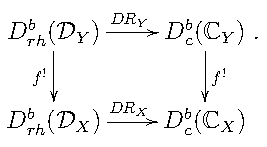
\includegraphics[width=0.2152\paperwidth]{images/L14-p124-pullback.pdf}\end{figure}
\begin{figure}[H]\centering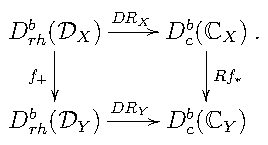
\includegraphics[width=0.2162\paperwidth]{images/L14-p124-direct.pdf}\end{figure}
特别地，即使$f$不是真映射，$\mathrm Rf_*$仍保持代数可构造性。
\end{enumerate}
\end{theorem}
\needspace{5\baselineskip}\section{第14讲参考文献}\label{L14S4}
\begin{references}
\refitem{L14bibPS}{PS} Chris A. M. Peters and Joseph H. M. Steenbrink, \emph{Mixed Hodge Structures}, Springer-Verlag Berlin Heidelberg, Ch. 13 \S13.3--\S13.6.
\refitem{L14bibB}{B} J. Bernstein, \emph{Algebraic Theory of D-modules}, available at\\ \url{http://www.math.columbia.edu/~khovanov/resources/Bernstein-dmod.pdf}.
\end{references}
